\documentclass[12pt]{article}

% Page geometry -- NBER style
\usepackage[margin=1in]{geometry}

% Font: Times New Roman
\usepackage{newtxtext,newtxmath}

% Double spacing
\usepackage{setspace}
\doublespacing

% Bibliography -- author-year
\usepackage[authoryear,round]{natbib}

% Tables
\usepackage{booktabs}
\usepackage{longtable}

% Figures
\usepackage{graphicx}

% Math
\usepackage{amsmath}

% Appendices
\usepackage[titletoc]{appendix}

% Captions
\usepackage{caption}

% Hyperlinks (load last)
\usepackage[hidelinks]{hyperref}

\title{Corporate Governance Reform and the Korea Discount:\\
Lessons from Japan's Reform Experience}
\author{[Author]}
\date{\today}

\begin{document}
\maketitle

\begin{abstract}
South Korean equities have traded at a persistent structural discount to developed-market peers
for over two decades. Using a 20-year monthly panel of index-level price-to-book (P/B) ratios
for KOSPI, TOPIX, S\&P~500, and MSCI~EM from 2004 to 2024, we document that the Korea Discount
averages $-0.177\times$ relative to TOPIX ($t=-3.23$; 95\% CI: $[-0.284\times, -0.069\times]$)
and $-0.601\times$ relative to MSCI~EM ($t=-10.30$). We use Japan's three staged corporate
governance reforms --- the Stewardship Code (February 2014), the Corporate Governance Code
(June 2015), and the Tokyo Stock Exchange P/B reform (March 2023) --- as policy benchmarks
rather than as clean natural experiments. A descriptive event-window analysis of the KOSPI--TOPIX P/B
spread shows large movements around the reform dates, but the implemented saturated
cohort-by-month design does not support conventional standard errors or causal inference.
Panel OLS with country and time fixed effects produces imprecise reform-by-Japan interactions:
wild-bootstrap $p$-values are 0.625, 0.375, and 0.500 for the three reforms, respectively,
given only $N=4$ country clusters. A demeaned synthetic-control exercise for the 2023 TSE
P/B reform assigns full weight to MSCI EM Asia (RMSPE = 0.1451); the post-reform gap does
not provide robust evidence of an idiosyncratic Japan governance premium after accounting
for regional equity momentum. The evidence therefore supports the existence of a persistent
Korea Discount, but it does not by itself identify the valuation gain Korea would realize
from adopting Japan-style reforms.
\end{abstract}

\newpage
\tableofcontents
\newpage

%% ============================================================
\section{Introduction}
\label{sec:intro}
%% ============================================================

South Korean equities occupy an anomalous position in global capital markets. Despite Korea's
membership in the G20, its well-developed export-oriented industrial base, and macroeconomic
fundamentals broadly comparable to other high-income economies, KOSPI Composite index-level
price-to-book ratios have persistently trailed those of comparable benchmarks for over two
decades. Over the 2004--2024 sample period, the KOSPI P/B ratio averaged $-0.177\times$ below
TOPIX ($t=-3.23$, 95\% CI: $[-0.284\times, -0.069\times]$) and $-0.601\times$ below MSCI~EM
($t=-10.30$, 95\% CI: $[-0.716\times, -0.486\times]$). This persistent, statistically
significant undervaluation --- the ``Korea Discount'' --- remains one of the most debated
puzzles in international equity valuation. Figure~\ref{fig:figure1} displays the full
20-year trajectory of KOSPI P/B relative to its benchmark peers.

\begin{figure}[htbp]
  \centering
  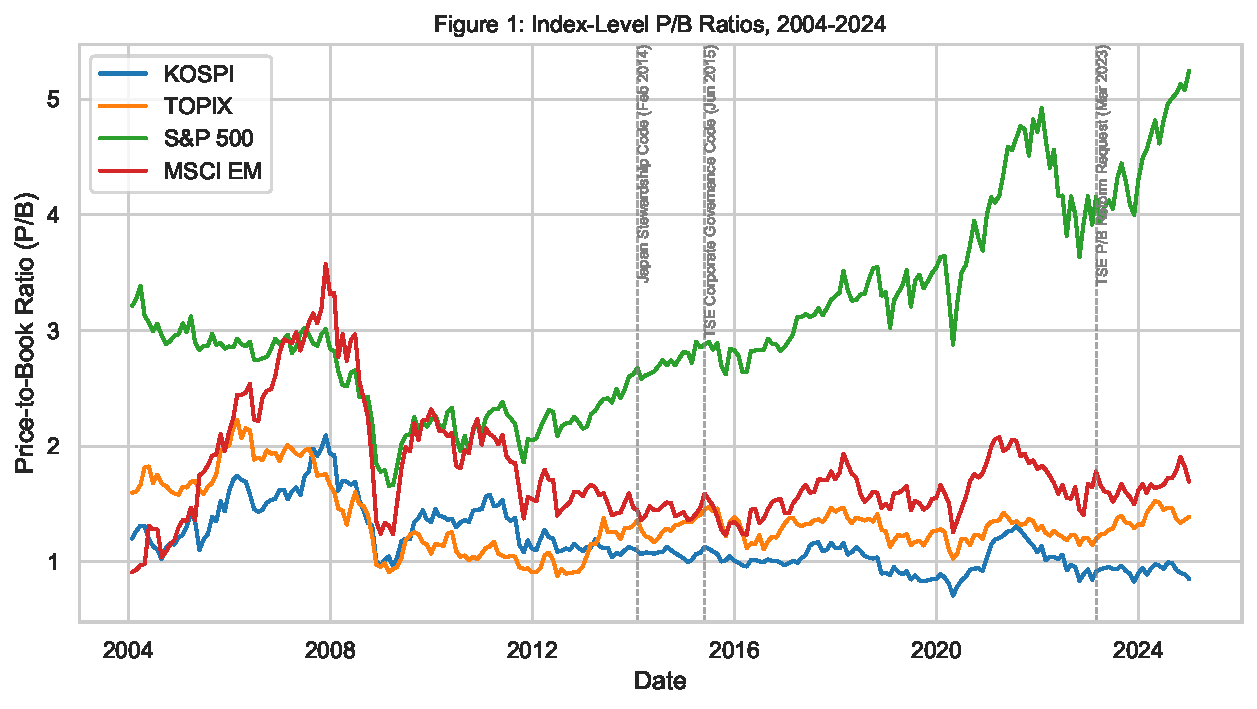
\includegraphics[width=\textwidth]{../output/figures/figure1_pb_comparison.pdf}
  \caption{Index-Level Price-to-Book Ratios, 2004--2024. KOSPI trades at a persistent discount
    to TOPIX, S\&P~500, and MSCI~EM throughout the sample period. The Korea Discount averages
    $-0.177\times$ relative to TOPIX ($t=-3.23$) and $-0.601\times$ relative to MSCI~EM
    ($t=-10.30$). Dashed vertical lines mark Japan's three governance reform dates
    (February 2014, June 2015, March 2023).}
  \label{fig:figure1}
\end{figure}

We emphasize three structural channels that plausibly account for the discount: (1) chaebol
cross-shareholding networks that generate governance opacity and suppress minority-shareholder
value; (2) a regulatory environment that historically afforded limited legal recourse to
outside investors; and (3) a geopolitical risk premium arising from North Korea's nuclear
program. Japan provides a useful policy benchmark, but not a clean source of causal
identification in the current data. Japan faced an analogous
valuation discount through much of the 2000s and 2010s and responded with three staged
governance reforms --- the Stewardship Code (February 2014), the Corporate Governance Code
(June 2015), and the Tokyo Stock Exchange P/B reform (March 2023). Korea did not implement
an equally forceful staggered program over the primary 2004--2024 sample, but Korea's own
Stewardship Code and 2024 Value-Up Program mean that a strict never-treated interpretation
would overstate the design.

This paper makes three contributions. First, we construct the first panel study using all
three Japan governance reform dates jointly as descriptive event windows for the KOSPI--TOPIX
valuation spread. This exercise documents timing and magnitude, while making explicit that
the saturated design and overlapping 2014--2015 windows do not deliver valid conventional
inference. Second, we report two-way fixed-effects panel estimates with small-cluster
wild-bootstrap $p$-values, showing that the reform interactions are too noisy to sustain
strong directional claims. Third, we provide a synthetic-control check for the 2023 TSE P/B
reform and transparently report the single-donor weight structure, which limits the strength
of the counterfactual interpretation.

Section~\ref{sec:litreview} surveys the prior literature and institutional background.
Section~\ref{sec:methodology} describes data, causal mechanisms, and identification strategy.
Section~\ref{sec:results} reports empirical results. Section~\ref{sec:discussion} discusses
limitations, policy implications, and conclusions. Appendices contain variable definitions
and robustness tables.

%% ============================================================
\section{Literature Review and Institutional Background}
\label{sec:litreview}
%% ============================================================

\subsection{The Korea Discount: Prior Evidence and the Chaebol Structure}

The Korea Discount has attracted a substantial body of academic and practitioner research.
South Korean corporate structure is dominated by \textit{chaebols} --- large, family-controlled
conglomerates that collectively account for a substantial share of KOSPI market capitalization
and national exports. The defining feature of the chaebol is a layered ownership architecture
in which a founding family holds a relatively small direct equity stake in each affiliate but
exercises effective control through a web of cross-shareholdings and pyramid ownership
\citep{claessens2000}. This generates a \textit{principal--principal} agency problem that is
analytically distinct from the classic principal--agent framework of \citet{jensen1976}: the
conflict is between the controlling family (a concentrated principal) and minority shareholders
(diffuse outside principals), with the family having both the incentive and means to extract
private benefits --- tunneling --- without bearing the proportionate economic cost.

\citet{baek2004} provide the foundational empirical paper on this mechanism. Exploiting the
1997 Korean financial crisis as an exogenous shock, they show that firms with greater
separation between control rights and cash-flow rights experienced larger equity value declines,
establishing that tunneling has quantifiable and economically large effects on market valuations.
\citet{claessens2000} document systematically across East Asian corporations that the median
Korean firm has a control-to-cash-flow ratio of approximately 2:1, highest in the region, and
that this separation is associated with a significant discount to Tobin's $q$.

\citet{black2006} construct a Korean corporate governance index (KCGI) using survey data on
board practices, disclosure, shareholder rights, and ownership structure, and show via panel
OLS that higher KCGI scores are associated with significantly higher Tobin's $q$ values ---
results that survive controls for firm size, leverage, profitability, and industry fixed
effects. \citet{kcmi2023} provide the most recent comprehensive assessment from the Korea
Capital Market Institute, identifying governance structure, low shareholder returns, market
accessibility deficiencies, and the inheritance tax structure (rates up to 60\%, applied to
market value, creating controlling-family incentives to keep share prices depressed) as the
four primary contributors.

An important methodological distinction separates prior work from this paper. The firm-level
literature identifies the cross-sectional governance--valuation relationship using firm-level
governance indices, but cannot readily estimate the causal effect of a nationwide governance
reform shock. Our event-study and panel designs fill this gap, at the cost of operating with
a single treated country ($N=1$) and the inferential challenges this entails.

\subsection{Japan's Governance Reforms and Their Empirical Literature}

Japan's governance reform program is the source of identifying variation for this study.
Japan faced a structurally similar valuation discount through the 2000s and 2010s, attributed
to cross-shareholding (\textit{keiretsu} networks), weak board independence, and low dividend
payout ratios. The government responded with three landmark interventions.

\textbf{Japan Stewardship Code (February 2014).} The Financial Services Agency introduced
Japan's Stewardship Code in February 2014, requiring institutional investors to adopt a
governance engagement policy and disclose voting rights exercise. The comply-or-explain
framework achieved high adoption among domestic and eventually foreign managers with Japanese
equity mandates. \citet{miyajima2023} document that the Code accelerated the unwinding of
cross-shareholding relationships: institutional investors now under formal obligation to
justify passive holdings of cross-held shares began pressing companies to restructure these
positions. Firms with larger cross-holding reductions experienced commensurately larger
improvements in Tobin's $q$.

\textbf{Corporate Governance Code (June 2015).} The Tokyo Stock Exchange and FSA jointly
introduced the Corporate Governance Code in June 2015, requiring all TSE-listed companies to
comply with governance principles or explain deviations. The code mandated at least two
independent outside directors --- a fundamental change for Japanese boards historically
composed almost entirely of long-serving inside managers \citep{eberhart2012}. By 2017,
over 90\% of JPX-Nikkei 400 constituents had appointed at least two independent directors.
\citet{eberhart2012} finds that transitions toward independent-director-inclusive boards are
associated with improvements in operating performance and, over longer horizons, equity
valuations.

\textbf{TSE P/B Reform (March 2023).} The Tokyo Stock Exchange's March 2023 ``Request for
Disclosure of Policies on Capital Cost and Stock Price Awareness'' instructed companies
trading below $1.0\times$ book value to disclose specific plans to improve capital efficiency.
Its impact was immediate: TOPIX P/B rose from approximately $1.0\times$ in early 2023 to
$1.36\times$ over the 2023--2024 post-reform period, while KOSPI P/B remained at approximately
$0.93\times$ --- widening the KOSPI--TOPIX spread.

All three reform dates are locked in \texttt{config.py} before any data transformation,
providing a look-ahead bias firewall: Stewardship Code 2014-02-01, Corporate Governance Code
2015-06-01, TSE P/B reform 2023-03-01.

Korea's own policy response is instructive for comparison. Korea adopted a Stewardship Code
in December 2016 (revised 2018), but it was widely assessed as weaker in enforcement than
Japan's 2014 equivalent --- the National Pension Service's engagement remained intermittent
and the comply-or-explain mechanism produced limited behavioral change. The \textit{Korea
Corporate Value-Up Program} (launched by the FSC in 2024) is modeled explicitly on the 2023
TSE P/B reform but remains voluntary; the FSC has proposed Commercial Act amendments
strengthening fiduciary duties to explicitly include minority shareholders. This reform
trajectory makes Korea a partial comparison case rather than a strictly never-treated unit.

\subsection{Corporate Governance, Legal Institutions, and Equity Valuation}

The broader governance--valuation literature provides the theoretical grounding for the Korea
Discount hypothesis. \citet{shleifer1997} survey the corporate governance literature and
document that ownership concentration, while potentially reducing manager--shareholder
conflicts, intensifies conflicts between controlling shareholders and minority investors ---
exactly the principal--principal problem that characterizes chaebols. Legal protection of
minority shareholders is established as a first-order determinant of equity valuations across
countries.

\citet{porta1998} and \citet{porta2002} establish the foundational law-and-finance framework:
countries with stronger statutory investor protections have larger, more liquid capital markets.
\citet{porta2002} show that investor protection is causally associated with higher dividend
yields and higher Tobin's $q$. The Korea Discount is a specific application of this framework:
Korea's civil-law tradition combined with the chaebol structure places it toward the
weak-investor-protection end of the international distribution. Japan's reform program
demonstrates that de facto governance practices can be improved through targeted regulatory
intervention even within a civil-law system. \citet{gompers2003} provide corroborating
evidence in the US context, showing that firms with stronger shareholder rights earn
significantly higher abnormal returns.

Specific legal deficiencies during the primary sample period in Korea include: high ownership
thresholds for minority shareholders to bring derivative suits; comparatively lax board
independence requirements relative to OECD peers (the Commercial Act did not mandate a
majority of independent directors until reforms beginning in 2020); related-party transaction
disclosure thresholds that permitted intragroup transactions without shareholder approval; and
shareholder proposal mechanisms requiring higher ownership thresholds than the US or UK.

\subsection{Geopolitical Risk}

A second structural channel is the country-specific risk premium arising from North Korea's
nuclear weapons and ballistic missile program. North Korea conducted six nuclear tests over
the sample period: October 2006, May 2009, February 2013, January 2016, September 2016, and
September 2017. The 2017 test, alongside ICBM launches demonstrating continental US range,
coincided with the largest single-period widening of the Korea--TOPIX P/B spread visible in
Figure~\ref{fig:figure1}. Unlike the governance channels, which in principle could be
eliminated through domestic policy reform, the geopolitical risk channel reflects an external
threat with no direct Korean government lever for short-term resolution.

The \citet{imf2021} GPRNK analysis finds that North Korean provocations primarily affect
systematic risk and market beta --- a level effect on the required return --- rather than
causing permanent cumulative discount widening following each escalation event. This suggests
the geopolitical risk premium is embedded in the structural discount level rather than
generating time-series variation. The empirical results in Section~\ref{sec:results} confirm
this interpretation: the GPR escalation coefficient is statistically insignificant at
conventional levels.

\subsection{Empirical Methods and Inference}

The empirical design is intentionally conservative. Staggered difference-in-differences
methods such as \citet{cengiz2019} and \citet{baker2022} motivate the concern that pooled
two-way fixed-effects estimators can be misleading when treatment effects differ across
cohorts. In this application, however, the data contain only one reforming country and three
events within that same country, with overlap between the 2014 and 2015 reform windows. The
event-window estimates are therefore presented as descriptive abnormal movements in the
KOSPI--TOPIX spread, not as a clean stacked DiD estimator.

The synthetic control of \citet{abadie2010} is designed for settings with a single treated
unit, but its credibility depends on pre-treatment fit, donor-pool plausibility, and a stable
weight structure. Wild-bootstrap inference \citep{cameron2008} with Rademacher weights is used
for the panel OLS interactions because asymptotic cluster-robust variance estimators perform
poorly with only $N=4$ country clusters. Even the wild bootstrap is limited in such a small
panel, so we report $p$-values alongside point estimates and avoid interpreting statistically
insignificant estimates as evidence of zero treatment effects.

%% ============================================================
\section{Methodology}
\label{sec:methodology}
%% ============================================================

\subsection{Data Sources and Variable Construction}

The primary data are monthly index-level price-to-book (P/B) ratios exported from the
Bloomberg Terminal using the Bloomberg Data License Historical Data Request protocol
(field code: \texttt{PX\_TO\_BOOK\_RATIO}), which reports aggregate market capitalization
divided by aggregate book value of equity across all index constituents, rebalanced at the
index's standard reconstitution frequency.

Four benchmark indices constitute the core panel: KOSPI Composite (Bloomberg ticker:
KOSPI Index), TOPIX (TPX Index), S\&P~500 (SPX Index), and MSCI~EM (MXEF Index). The primary
analysis sample spans January 2004 to December 2024 --- 252 calendar months per series ---
yielding 1,008 country-month observations. The processed panel stored on disk includes
additional observations through April 2026, for 1,072 rows, because the raw extracts were
updated after the primary paper window. All Bloomberg raw CSV exports are version-controlled
in \texttt{data/raw/} with provenance documented in \texttt{data/raw/MANIFEST.md} (vintage
date: 2026-04-20).

We prefer P/B over price-to-earnings (P/E) for three reasons: (i) book value is considerably
less cyclically volatile than earnings, making P/B a more stable measure of structural
discount; (ii) book value does not go negative for index-level aggregates, avoiding the
sign-change problem during recessions; and (iii) the TSE P/B reform and Korea's Value-Up
Program are explicitly framed in P/B terms. P/E robustness results are presented in
Appendix~B; results are qualitatively consistent but noisier.

The canonical panel has schema (\texttt{date}, \texttt{country}, \texttt{pb}, \texttt{pe},
\texttt{fx\_rate}), stored as \texttt{data/processed/panel.parquet}. The Geopolitical Risk index
\citep{caldara2022}, with the Korea-specific GPRNK sub-index \citep{imf2021} isolating North
Korean escalation events, is sourced at monthly frequency and complete over the full sample
period. All four monthly P/B series are complete with no gaps.

The use of official, published index-level P/B series substantially mitigates survivorship
bias concerns: P/B ratios are computed by the index provider over all constituents as of
each month-end, including firms that subsequently exit. Index constituent turnover is a
potential source of composition bias if lower-valuation firms are systematically replaced
by higher-valuation entrants, but the Korea Discount has \textit{persisted} despite constituent
turnover, and the 2008--2009 global financial crisis P/B compression affects all four series
simultaneously in a manner consistent with known economic events --- providing a cross-market
consistency check.

\begin{table}
\caption{Summary statistics of index-level P/B ratios by country and sub-period.}
\label{tab:summary_stats}
\begin{tabular}{llrrrrr}
\toprule
 & Period & mean & median & std & min & max \\
country &  &  &  &  &  &  \\
\midrule
KOSPI & Full (2004--2024) & 1.18 & 1.10 & 0.26 & 0.71 & 2.09 \\
MSCI\_EM & Full (2004--2024) & 1.78 & 1.65 & 0.47 & 0.91 & 3.58 \\
SP500 & Full (2004--2024) & 3.08 & 2.89 & 0.81 & 1.66 & 5.25 \\
TOPIX & Full (2004--2024) & 1.35 & 1.31 & 0.28 & 0.88 & 2.23 \\
KOSPI & Pre-reform (2004--2013) & 1.36 & 1.34 & 0.25 & 0.96 & 2.09 \\
MSCI\_EM & Pre-reform (2004--2013) & 1.97 & 1.91 & 0.60 & 0.91 & 3.58 \\
SP500 & Pre-reform (2004--2013) & 2.51 & 2.42 & 0.40 & 1.66 & 3.39 \\
TOPIX & Pre-reform (2004--2013) & 1.41 & 1.29 & 0.39 & 0.88 & 2.23 \\
KOSPI & Reform era (2014--2022) & 1.02 & 1.03 & 0.12 & 0.71 & 1.31 \\
MSCI\_EM & Reform era (2014--2022) & 1.59 & 1.55 & 0.20 & 1.24 & 2.08 \\
SP500 & Reform era (2014--2022) & 3.39 & 3.28 & 0.63 & 2.58 & 4.92 \\
TOPIX & Reform era (2014--2022) & 1.29 & 1.28 & 0.10 & 1.03 & 1.48 \\
KOSPI & Post-TSE (2023--2024) & 0.93 & 0.94 & 0.04 & 0.83 & 1.00 \\
MSCI\_EM & Post-TSE (2023--2024) & 1.66 & 1.66 & 0.10 & 1.50 & 1.91 \\
SP500 & Post-TSE (2023--2024) & 4.51 & 4.47 & 0.43 & 3.91 & 5.25 \\
TOPIX & Post-TSE (2023--2024) & 1.36 & 1.35 & 0.10 & 1.15 & 1.53 \\
\bottomrule
\end{tabular}
\end{table}

% Korea Discount magnitude - auto-generated by discount_stats.py
% Usage in LaTeX: \korDiscountTOPIX, \korDiscountMSCIEM, etc.
%
\newcommand{\korDiscountTOPIX}{-0.177x}
\newcommand{\korDiscountTOPIXTStat}{-3.23}
\newcommand{\korDiscountTOPIXCILower}{-0.284x}
\newcommand{\korDiscountTOPIXCIUpper}{-0.069x}
%
\newcommand{\korDiscountMSCIEM}{-0.601x}
\newcommand{\korDiscountMSCIEMTStat}{-10.30}
\newcommand{\korDiscountMSCIEMCILower}{-0.716x}
\newcommand{\korDiscountMSCIEMCIUpper}{-0.486x}
%


\subsection{Causal Mechanisms}

The Korea Discount reflects three compounding structural channels, each of which independently
suppresses the equity valuation that international investors assign to KOSPI.

\textbf{Chaebol Opacity and Agency Costs.} Chaebol-affiliated firms represent the substantial
majority of KOSPI market capitalization. The principal--principal agency problem arising from
the control-to-cash-flow wedge generates three distinct opacity mechanisms: intragroup
related-party transactions that are difficult to assess from public disclosures; group-level
accounting that obscures individual entity economics; and controlling-family incentives to
keep equity prices depressed during generational wealth transfers, given inheritance tax rates
up to 60\% applied to market value. The ``double-counting'' problem in index-level valuation
--- where both parent companies and multiple listed subsidiaries appear in KOSPI --- adds a
mechanical book-value inflation that international investors must discount.

\textbf{Minority Shareholder Recourse Deficit.} The legal deficiencies described in
Section~\ref{sec:litreview} collectively reduce the expected return that minority shareholders
can extract from KOSPI-listed firms. Following \citet{porta1998, porta2002}, weak statutory
investor protections are associated with lower equity valuations across countries. Korea's
position toward the weak-protection end of the international distribution during 2004--2024
generates a commensurate valuation penalty.

\textbf{Geopolitical Risk Premium.} The tail risk of armed conflict on the Korean peninsula
warrants a discount to intrinsic value not shared by TOPIX, S\&P~500, or MSCI~EM. Even a
small probability of catastrophic loss justifies a meaningful discount to expected-cash-flow-based
valuations. As noted in Section~\ref{sec:litreview} and confirmed empirically in
Section~\ref{sec:results}, this premium appears to be priced continuously as a level discount
rather than reacting discretely to individual escalation events.

The interaction of these three channels creates a cumulative discount exceeding what any
individual channel would predict in isolation.

\subsection{Empirical Strategy}

This paper uses three empirical exercises with different evidentiary weight. The headline
discount statistics establish the magnitude and persistence of the Korea Discount. A
descriptive event-window analysis and two-way fixed-effects panel OLS examine whether Japan's
reform dates line up with changes in the KOSPI--TOPIX valuation spread. A synthetic-control
exercise evaluates the 2023 TSE P/B reform against regional peers. All reform dates are fixed
in \texttt{config.py} before any data transformation.

\subsubsection{Descriptive Event-Window Analysis}

The implemented event-window exercise is not a conventional stacked difference-in-differences
estimator. For each Japan reform date $k \in \{2014, 2015, 2023\}$, we construct the monthly
spread between Korea and Japan:

\begin{equation}
  S_t = PB^{KOSPI}_t - PB^{TOPIX}_t .
  \label{eq:spread}
\end{equation}

Within each cohort, the script estimates a linear pre-event trend in $S_t$ over the
$[-36,-1]$ month window and defines abnormal spread movement as the observed spread less this
pre-event trend. The reported coefficient at event month $\tau$ is the abnormal spread at
that month, and the reported CAR is the cumulative sum of these monthly abnormal spread
movements over the displayed $[-12,+24]$ window:

\begin{equation}
  CAR_{\tau,k} = \sum_{s=-12}^{\tau} \left(S_{t_k+s} - \widehat{S}_{t_k+s}^{pretrend}\right).
  \label{eq:event_car}
\end{equation}

The sign convention is therefore important: a positive CAR means the KOSPI--TOPIX spread rose
relative to its pre-event trend, not that Japan's P/B rose. A negative CAR means the Korea
discount versus TOPIX deepened relative to the fitted pre-event trend. The design is saturated
at the cohort-by-relative-month level; conventional sandwich standard errors are undefined,
so the event-window results are interpreted descriptively. The 2014 and 2015 windows also
overlap, so those two cohorts are not independent reform experiments.

\subsubsection{Panel OLS}

As a complementary approach, we estimate a two-way fixed effects panel OLS specification
using the full country-month panel:

\begin{equation}
  Y_{ct} = \alpha_c + \alpha_t + \sum_{k} \beta_k \cdot D_{kt} \cdot \mathbf{1}[c = \text{Japan}] + \varepsilon_{ct}
  \label{eq:panel_ols}
\end{equation}

where $D_{kt} = \mathbf{1}[\text{date} \geq \text{reform\_date}_k]$ and the three
reform-by-Japan interaction terms $\beta_k$ are the parameters of interest. The specification
is estimated via \texttt{linearmodels.PanelOLS} in Python with entity and time fixed effects
absorbed by within-demeaning. Inference uses wild-bootstrap with 999 Rademacher draws,
clustered by country \citep{cameron2008}.

\subsubsection{Synthetic Control}

Following \citet{abadie2010}, we apply the synthetic control method to the 2023 TSE P/B
reform, the event with the most direct P/B mandate. The synthetic control constructs a convex
weighted combination of donor markets (MSCI EM, MSCI EM Asia, MSCI HK, MSCI Taiwan, MSCI
China, MSCI India, MSCI Indonesia) minimizing the pre-treatment mean squared prediction error
(MSPE) on demeaned TOPIX P/B. Demeaning by each unit's pre-treatment mean resolves a convex
hull boundary problem caused by Japan's structurally low absolute valuation level relative to
regional peers. KOSPI is excluded from the donor pool to avoid using the paper's primary
comparison market as part of the Japan counterfactual. The post-treatment gap --- actual
demeaned TOPIX P/B minus synthetic demeaned TOPIX P/B --- is interpreted as a diagnostic for
whether Japan outperformed comparable regional equity markets after the 2023 reform; given
the single treated unit and the realized single-donor solution, it should not be read as a
stand-alone causal estimate.

%% ============================================================
\section{Results}
\label{sec:results}
%% ============================================================

We report results from the descriptive event-window analysis, panel OLS, geopolitical risk
sub-analysis, and synthetic control. All analyses use price-to-book as the primary outcome
variable.

\subsection{Descriptive Event-Window Analysis}

Figure~\ref{fig:figure2} displays the three event-window CAR series, and
Table~\ref{tab:event_study_coefs} reports the monthly coefficients and CARs underlying the
figure. These are descriptive abnormal movements in the KOSPI--TOPIX P/B spread, not
country-level treatment effects.

The 2014 Stewardship Code window shows a negative pre-event CAR that reverses after the event,
reaching approximately $+4.29$ by $\tau=+24$. Under the implemented sign convention, this
means the KOSPI--TOPIX spread rose relative to the fitted pre-event trend. The 2015 Corporate
Governance Code window displays a similar positive cumulative spread movement, reaching
approximately $+7.83$ by $\tau=+24$, but this window overlaps heavily with the 2014 reform
window and should not be interpreted as an independent causal experiment. The 2023 TSE P/B
Reform window moves in the opposite direction: CARs become persistently negative after the
announcement and reach approximately $-6.48$ by $\tau=+24$, indicating that the Korea discount
versus TOPIX deepened relative to the pre-event trend.

These patterns are useful for describing timing and magnitude. They do not establish that
Japan's governance reforms caused valuation convergence, and they do not imply that all three
reform windows point in the same direction.

\begin{figure}[htbp]
  \centering
  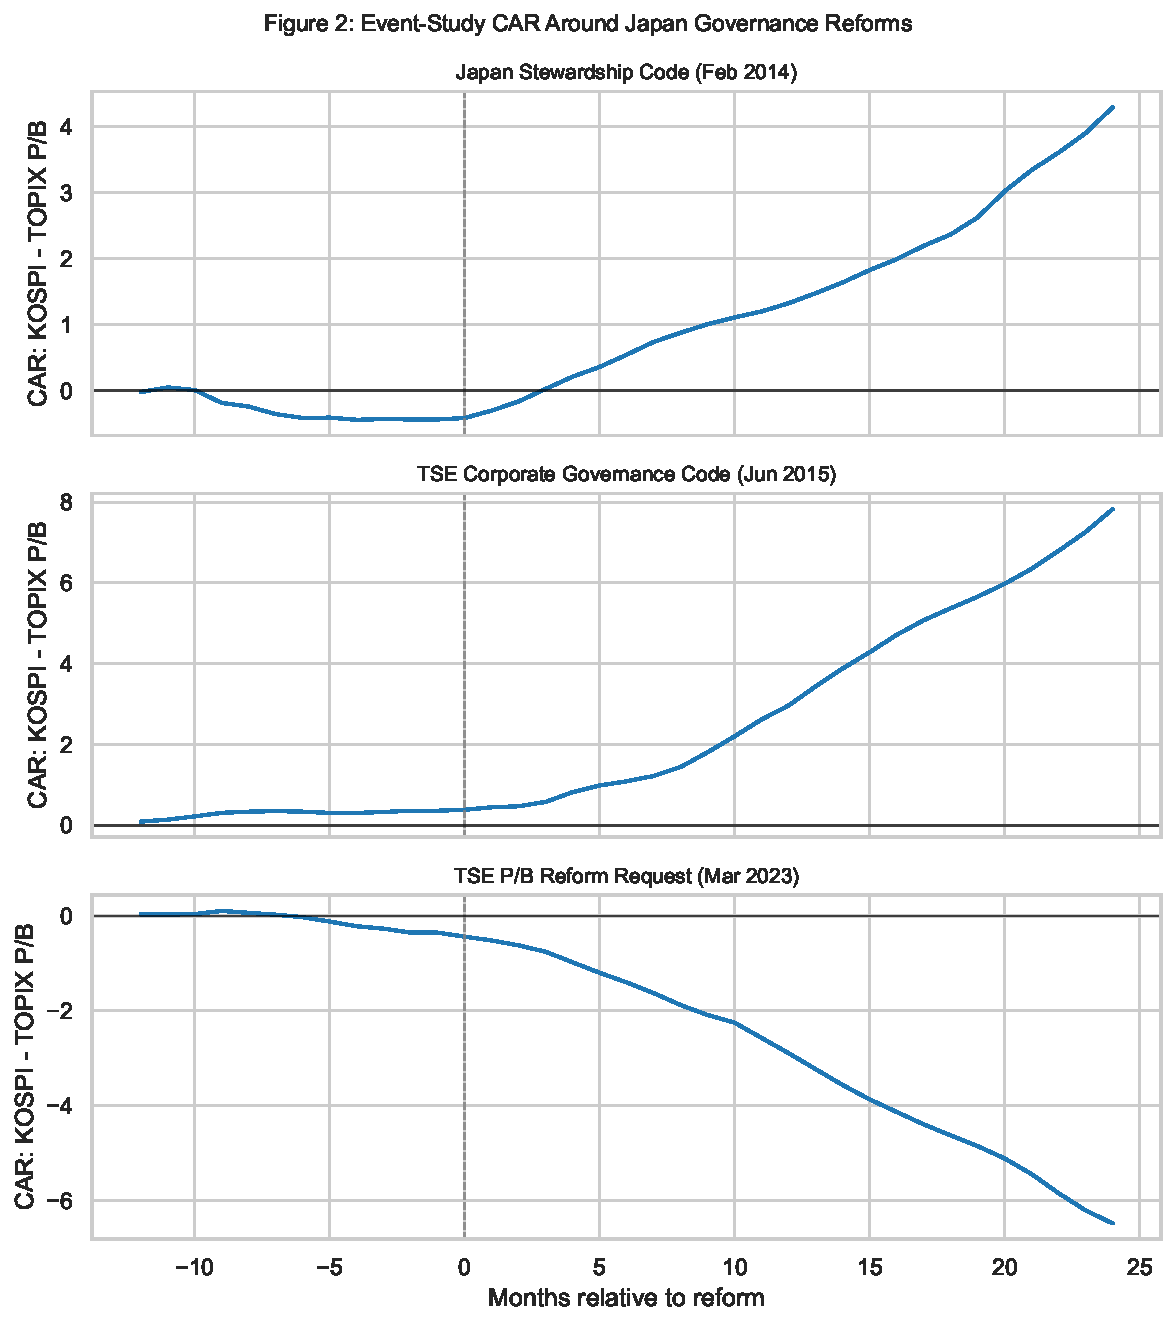
\includegraphics[width=\textwidth]{../output/figures/figure2_event_study.pdf}
  \caption{Descriptive Event-Window CARs Around Japan Reform Dates. Three panels show
    cumulative abnormal movements in the KOSPI--TOPIX P/B spread for the 2014 Stewardship
    Code, 2015 Corporate Governance Code, and 2023 TSE P/B Reform windows. The displayed CARs
    are based on a pre-event spread trend and are reported without confidence intervals.}
  \label{fig:figure2}
\end{figure}

% Descriptive CARs: coefficients and cumulative abnormal KOSPI-TOPIX P/B spread.
% Standard errors are not reported: the saturated cohort x relative-time design
% makes sandwich robust inference undefined. See paper text for robustness discussion.
\begin{table}
\caption{Stacked event-study descriptive CAR estimates (no inference reported).}
\label{tab:event_study_coefs}
\begin{tabular}{lrrr}
\toprule
Event & Month & Coefficient & CAR \\
\midrule
Japan Stewardship Code (Feb 2014) & -12 & -0.02 & -0.02 \\
Japan Stewardship Code (Feb 2014) & -11 & 0.07 & 0.05 \\
Japan Stewardship Code (Feb 2014) & -10 & -0.04 & 0.01 \\
Japan Stewardship Code (Feb 2014) & -9 & -0.19 & -0.19 \\
Japan Stewardship Code (Feb 2014) & -8 & -0.06 & -0.24 \\
Japan Stewardship Code (Feb 2014) & -7 & -0.11 & -0.36 \\
Japan Stewardship Code (Feb 2014) & -6 & -0.06 & -0.42 \\
Japan Stewardship Code (Feb 2014) & -5 & 0.00 & -0.41 \\
Japan Stewardship Code (Feb 2014) & -4 & -0.03 & -0.44 \\
Japan Stewardship Code (Feb 2014) & -3 & 0.01 & -0.43 \\
Japan Stewardship Code (Feb 2014) & -2 & -0.01 & -0.44 \\
Japan Stewardship Code (Feb 2014) & -1 & 0.00 & -0.44 \\
Japan Stewardship Code (Feb 2014) & 0 & 0.02 & -0.42 \\
Japan Stewardship Code (Feb 2014) & 1 & 0.11 & -0.30 \\
Japan Stewardship Code (Feb 2014) & 2 & 0.14 & -0.17 \\
Japan Stewardship Code (Feb 2014) & 3 & 0.19 & 0.02 \\
Japan Stewardship Code (Feb 2014) & 4 & 0.18 & 0.21 \\
Japan Stewardship Code (Feb 2014) & 5 & 0.15 & 0.36 \\
Japan Stewardship Code (Feb 2014) & 6 & 0.18 & 0.54 \\
Japan Stewardship Code (Feb 2014) & 7 & 0.19 & 0.74 \\
Japan Stewardship Code (Feb 2014) & 8 & 0.14 & 0.88 \\
Japan Stewardship Code (Feb 2014) & 9 & 0.13 & 1.00 \\
Japan Stewardship Code (Feb 2014) & 10 & 0.10 & 1.11 \\
Japan Stewardship Code (Feb 2014) & 11 & 0.09 & 1.20 \\
Japan Stewardship Code (Feb 2014) & 12 & 0.12 & 1.32 \\
Japan Stewardship Code (Feb 2014) & 13 & 0.15 & 1.47 \\
Japan Stewardship Code (Feb 2014) & 14 & 0.16 & 1.64 \\
Japan Stewardship Code (Feb 2014) & 15 & 0.19 & 1.82 \\
Japan Stewardship Code (Feb 2014) & 16 & 0.16 & 1.99 \\
Japan Stewardship Code (Feb 2014) & 17 & 0.20 & 2.19 \\
Japan Stewardship Code (Feb 2014) & 18 & 0.17 & 2.36 \\
Japan Stewardship Code (Feb 2014) & 19 & 0.26 & 2.62 \\
Japan Stewardship Code (Feb 2014) & 20 & 0.40 & 3.02 \\
Japan Stewardship Code (Feb 2014) & 21 & 0.32 & 3.34 \\
Japan Stewardship Code (Feb 2014) & 22 & 0.26 & 3.60 \\
Japan Stewardship Code (Feb 2014) & 23 & 0.30 & 3.90 \\
Japan Stewardship Code (Feb 2014) & 24 & 0.39 & 4.29 \\
TSE Corporate Governance Code (Jun 2015) & -12 & 0.09 & 0.09 \\
TSE Corporate Governance Code (Jun 2015) & -11 & 0.05 & 0.14 \\
TSE Corporate Governance Code (Jun 2015) & -10 & 0.08 & 0.22 \\
TSE Corporate Governance Code (Jun 2015) & -9 & 0.09 & 0.31 \\
TSE Corporate Governance Code (Jun 2015) & -8 & 0.03 & 0.33 \\
TSE Corporate Governance Code (Jun 2015) & -7 & 0.01 & 0.35 \\
TSE Corporate Governance Code (Jun 2015) & -6 & -0.01 & 0.33 \\
TSE Corporate Governance Code (Jun 2015) & -5 & -0.03 & 0.30 \\
TSE Corporate Governance Code (Jun 2015) & -4 & -0.00 & 0.30 \\
TSE Corporate Governance Code (Jun 2015) & -3 & 0.02 & 0.33 \\
TSE Corporate Governance Code (Jun 2015) & -2 & 0.03 & 0.36 \\
TSE Corporate Governance Code (Jun 2015) & -1 & 0.00 & 0.36 \\
TSE Corporate Governance Code (Jun 2015) & 0 & 0.03 & 0.38 \\
TSE Corporate Governance Code (Jun 2015) & 1 & 0.06 & 0.44 \\
TSE Corporate Governance Code (Jun 2015) & 2 & 0.03 & 0.47 \\
TSE Corporate Governance Code (Jun 2015) & 3 & 0.11 & 0.58 \\
TSE Corporate Governance Code (Jun 2015) & 4 & 0.24 & 0.82 \\
TSE Corporate Governance Code (Jun 2015) & 5 & 0.16 & 0.98 \\
TSE Corporate Governance Code (Jun 2015) & 6 & 0.10 & 1.09 \\
TSE Corporate Governance Code (Jun 2015) & 7 & 0.13 & 1.22 \\
TSE Corporate Governance Code (Jun 2015) & 8 & 0.22 & 1.44 \\
TSE Corporate Governance Code (Jun 2015) & 9 & 0.37 & 1.81 \\
TSE Corporate Governance Code (Jun 2015) & 10 & 0.40 & 2.20 \\
TSE Corporate Governance Code (Jun 2015) & 11 & 0.42 & 2.62 \\
TSE Corporate Governance Code (Jun 2015) & 12 & 0.34 & 2.97 \\
TSE Corporate Governance Code (Jun 2015) & 13 & 0.47 & 3.44 \\
TSE Corporate Governance Code (Jun 2015) & 14 & 0.44 & 3.88 \\
TSE Corporate Governance Code (Jun 2015) & 15 & 0.40 & 4.28 \\
TSE Corporate Governance Code (Jun 2015) & 16 & 0.43 & 4.71 \\
TSE Corporate Governance Code (Jun 2015) & 17 & 0.36 & 5.08 \\
TSE Corporate Governance Code (Jun 2015) & 18 & 0.30 & 5.37 \\
TSE Corporate Governance Code (Jun 2015) & 19 & 0.29 & 5.66 \\
TSE Corporate Governance Code (Jun 2015) & 20 & 0.32 & 5.98 \\
TSE Corporate Governance Code (Jun 2015) & 21 & 0.37 & 6.35 \\
TSE Corporate Governance Code (Jun 2015) & 22 & 0.45 & 6.80 \\
TSE Corporate Governance Code (Jun 2015) & 23 & 0.47 & 7.26 \\
TSE Corporate Governance Code (Jun 2015) & 24 & 0.57 & 7.83 \\
TSE P/B Reform Request (Mar 2023) & -12 & 0.03 & 0.03 \\
TSE P/B Reform Request (Mar 2023) & -11 & -0.00 & 0.03 \\
TSE P/B Reform Request (Mar 2023) & -10 & 0.01 & 0.04 \\
TSE P/B Reform Request (Mar 2023) & -9 & 0.07 & 0.11 \\
TSE P/B Reform Request (Mar 2023) & -8 & -0.04 & 0.07 \\
TSE P/B Reform Request (Mar 2023) & -7 & -0.04 & 0.03 \\
TSE P/B Reform Request (Mar 2023) & -6 & -0.05 & -0.03 \\
TSE P/B Reform Request (Mar 2023) & -5 & -0.09 & -0.12 \\
TSE P/B Reform Request (Mar 2023) & -4 & -0.10 & -0.22 \\
TSE P/B Reform Request (Mar 2023) & -3 & -0.05 & -0.27 \\
TSE P/B Reform Request (Mar 2023) & -2 & -0.08 & -0.35 \\
TSE P/B Reform Request (Mar 2023) & -1 & 0.00 & -0.35 \\
TSE P/B Reform Request (Mar 2023) & 0 & -0.08 & -0.44 \\
TSE P/B Reform Request (Mar 2023) & 1 & -0.08 & -0.52 \\
TSE P/B Reform Request (Mar 2023) & 2 & -0.10 & -0.62 \\
TSE P/B Reform Request (Mar 2023) & 3 & -0.13 & -0.75 \\
TSE P/B Reform Request (Mar 2023) & 4 & -0.22 & -0.98 \\
TSE P/B Reform Request (Mar 2023) & 5 & -0.22 & -1.20 \\
TSE P/B Reform Request (Mar 2023) & 6 & -0.20 & -1.40 \\
TSE P/B Reform Request (Mar 2023) & 7 & -0.22 & -1.63 \\
TSE P/B Reform Request (Mar 2023) & 8 & -0.25 & -1.88 \\
TSE P/B Reform Request (Mar 2023) & 9 & -0.21 & -2.09 \\
TSE P/B Reform Request (Mar 2023) & 10 & -0.16 & -2.25 \\
TSE P/B Reform Request (Mar 2023) & 11 & -0.32 & -2.57 \\
TSE P/B Reform Request (Mar 2023) & 12 & -0.32 & -2.89 \\
TSE P/B Reform Request (Mar 2023) & 13 & -0.34 & -3.23 \\
TSE P/B Reform Request (Mar 2023) & 14 & -0.33 & -3.56 \\
TSE P/B Reform Request (Mar 2023) & 15 & -0.30 & -3.87 \\
TSE P/B Reform Request (Mar 2023) & 16 & -0.26 & -4.13 \\
TSE P/B Reform Request (Mar 2023) & 17 & -0.26 & -4.39 \\
TSE P/B Reform Request (Mar 2023) & 18 & -0.23 & -4.63 \\
TSE P/B Reform Request (Mar 2023) & 19 & -0.23 & -4.85 \\
TSE P/B Reform Request (Mar 2023) & 20 & -0.26 & -5.11 \\
TSE P/B Reform Request (Mar 2023) & 21 & -0.33 & -5.44 \\
TSE P/B Reform Request (Mar 2023) & 22 & -0.40 & -5.85 \\
TSE P/B Reform Request (Mar 2023) & 23 & -0.36 & -6.21 \\
TSE P/B Reform Request (Mar 2023) & 24 & -0.27 & -6.48 \\
\bottomrule
\end{tabular}
\end{table}


\subsection{Panel OLS}

Table~\ref{tab:panel_ols} reports the two-way fixed effects panel OLS results. The
reform-by-Japan interaction estimates are: Stewardship Code $\times$ Japan $= +0.09$
[$p = 0.625$]; Corporate Governance Code $\times$ Japan $= -0.32$ [$p = 0.375$]; TSE P/B
Reform $\times$ Japan $= -0.23$ [$p = 0.500$]. Bracketed values are wild-bootstrap $p$-values
(999 Rademacher draws, clustered by country), not standard errors.

These estimates are not robust evidence of a positive Japan governance re-rating effect.
Two of the three point estimates are negative, and none of the three reform-by-Japan
interactions achieves conventional significance under the small-cluster wild bootstrap. With
only $N=4$ country clusters, the panel OLS specification has severely limited statistical
power. We therefore interpret the panel estimates as a caution against over-reading the
Japan reform narrative in this country-level panel, not as primary causal evidence.

\begin{table}
\caption{Two-way fixed effects PanelOLS estimates of Japan reform valuation responses.}
\label{tab:panel_ols}
\begin{tabular}{llll}
\toprule
 & Baseline two-way FE & + reform dummies & + reform x Japan \\
term &  &  &  \\
\midrule
post\_stewardship &  & absorbed by time FE & absorbed by time FE \\
post\_cgc &  & absorbed by time FE & absorbed by time FE \\
post\_tse\_pb\_reform &  & absorbed by time FE & absorbed by time FE \\
stewardship\_x\_japan &  &  & 0.09 [0.625] \\
cgc\_x\_japan &  &  & -0.32 [0.375] \\
tse\_pb\_reform\_x\_japan &  &  & -0.23 [0.500] \\
log\_fx & -0.02 (0.01) & -0.02 (0.01) & -0.01 (0.01) \\
\multicolumn{4}{l}{\footnotesize Note: Coefficients from two-way FE PanelOLS. For \textit{+ reform x Japan} specification, bracketed values are wild-bootstrap p-values (999 Rademacher draws, clustered by country). Standard errors shown for all other estimable cells.} \\
\bottomrule
\end{tabular}
\end{table}


\subsection{Geopolitical Risk Sub-Analysis}

Table~\ref{tab:geo_risk} reports results from the geopolitical risk sub-analysis. The GPR
escalation coefficient is $-0.02$ ($t = -0.84$, $p = 0.40$) --- statistically insignificant
at conventional levels, consistent with the interpretation from Section~\ref{sec:litreview}
that markets price geopolitical risk continuously as a level discount rather than reacting
to individual escalation events. The TOPIX P/B coefficient is $+0.63$ ($t = 5.40$), capturing
the broader governance valuation convergence over the sample period.

Two caveats apply. First, the GPR escalation dummy may be correlated with global risk-off
episodes, as North Korean escalation events tend to cluster during periods of heightened
global geopolitical uncertainty. Second, the monthly panel frequency may be insufficient to
detect ephemeral reactions that resolve within weeks. Either interpretation is consistent with
\citet{imf2021}, who find that North Korean provocations primarily affect systematic risk and
market beta rather than generating permanent cumulative P/B spread widening.

\begin{figure}[htbp]
  \centering
  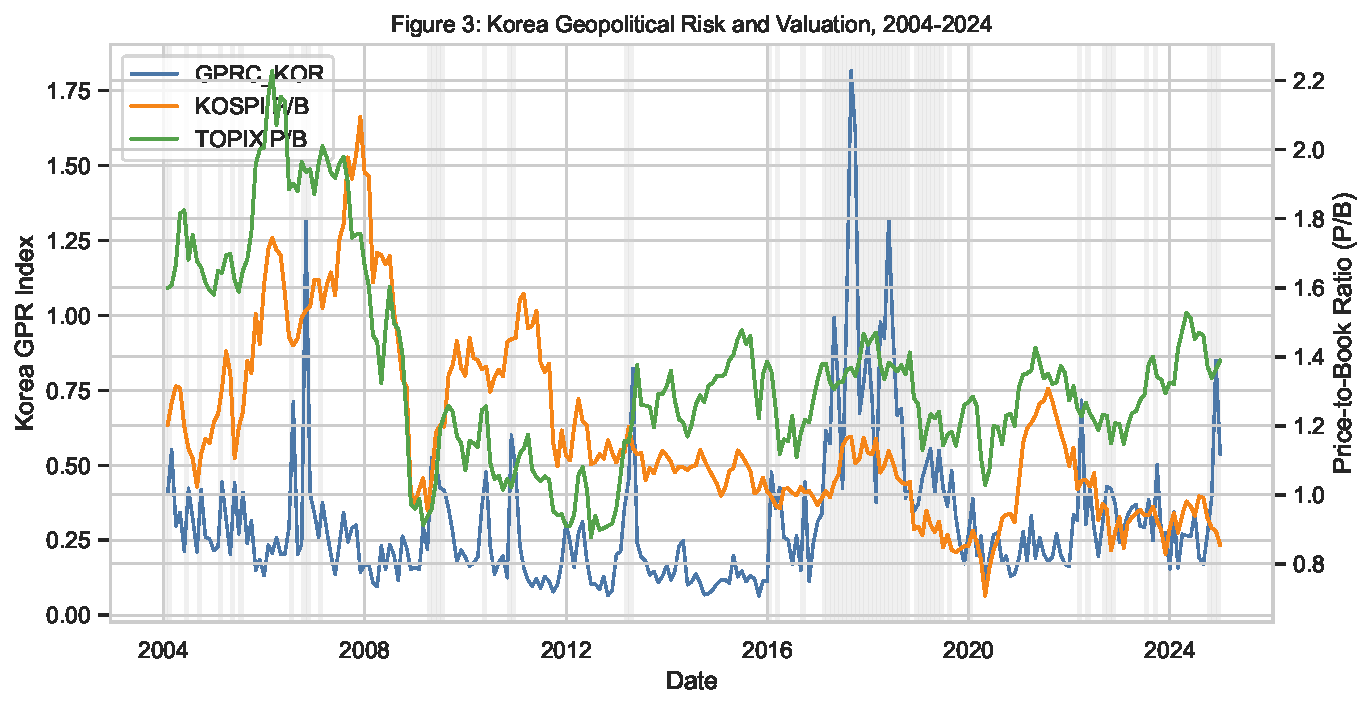
\includegraphics[width=\textwidth]{../output/figures/figure3_geo_risk.pdf}
  \caption{Geopolitical Risk Overlay: GPR Index and KOSPI P/B. The Caldara--Iacoviello
    Geopolitical Risk index (\citealt{caldara2022}) is overlaid against the KOSPI--TOPIX
    P/B spread. Shaded regions indicate North Korea escalation events above the 75th
    percentile of the GPR series. GPR escalation coefficient: $-0.02$ ($t = -0.84$,
    $p = 0.40$), statistically insignificant.}
  \label{fig:figure3}
\end{figure}

% Geo-risk regression table - auto-generated by geo_risk.py
\begin{table}[htbp]
\centering
\caption{Korea Geopolitical Risk and KOSPI Valuation}
\begin{tabular}{lrrrr}
\toprule
Term & Estimate & Std. Error & t-stat & p-value \\
\midrule
GPR escalation dummy & -0.02 & 0.02 & -0.84 & 0.40 \\
TOPIX P/B & 0.63 & 0.12 & 5.40 & 0.00 \\
\bottomrule
\end{tabular}
\begin{flushleft}\footnotesize N = 252 monthly observations. Year fixed effects included. GPR escalation threshold = 0.37. Partial identification caveat: the GPR-Korea escalation coefficient is an association, not a pure causal effect, because GPRC_KOR may also capture global risk-off episodes.\end{flushleft}
\end{table}


\subsection{Synthetic Control}

Figure~\ref{fig:synth} displays the synthetic control gap series for the 2023 TSE P/B Reform.
The optimization assigns full weight to MSCI EM Asia (weight $=1.0$), with pre-treatment
RMSPE of $0.1451$. The fit is close to the project threshold of $0.15$, but the single-donor
solution means the exercise is best interpreted as a comparison between Japan and MSCI EM
Asia after demeaning, not as a diversified synthetic portfolio.

The post-March-2023 gap series complicates the simple Japan reform narrative. TOPIX P/B rose
in absolute terms after the reform, but Japan did not cleanly break away from the regional
benchmark. The average post-reform gap through 2024 remains modestly positive, while the
first 18-month change in the gap is slightly negative ($-0.0028$ per month). This implies
that Japan's relative advantage over the synthetic benchmark faded rather than widened
monotonically. The observed TOPIX lift may therefore reflect a combination of governance
attention, regional equity momentum, yen depreciation, and broader risk appetite; the
country-level synthetic-control result does not isolate a purely idiosyncratic governance
premium.

\begin{figure}[htbp]
  \centering
  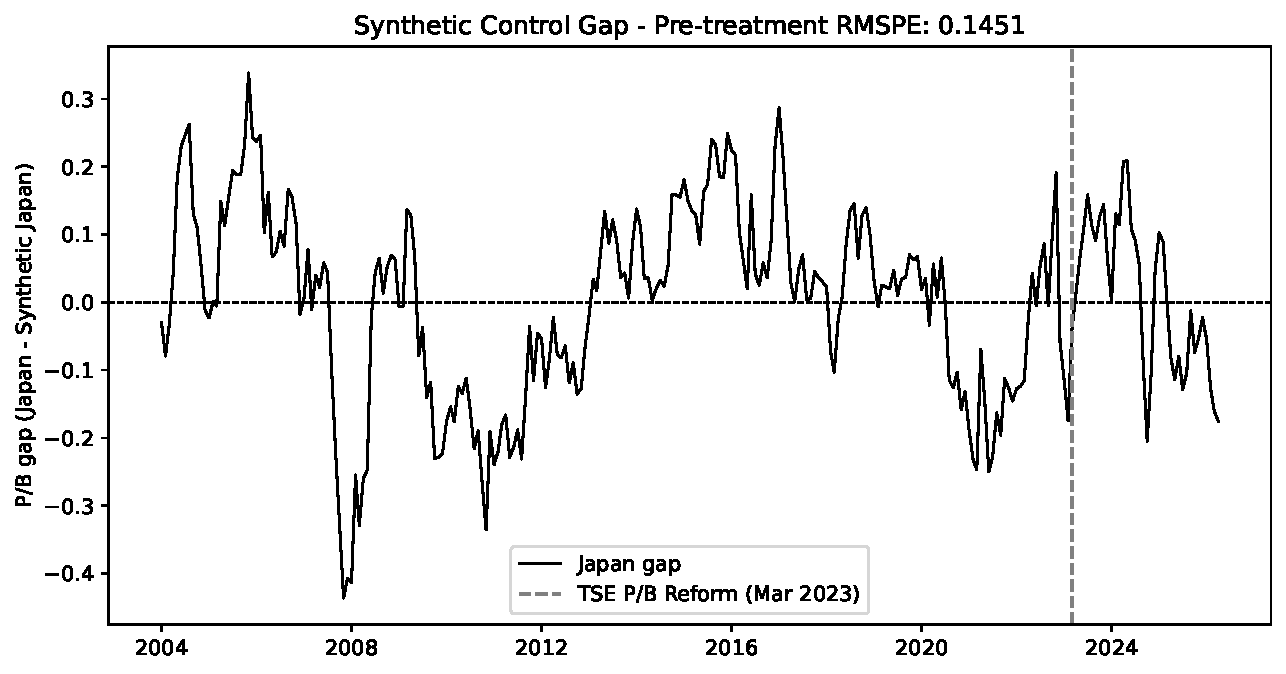
\includegraphics[width=\textwidth]{../output/figures/figure_synth_gap.pdf}
  \caption{Synthetic Control Gap: Japan P/B minus Synthetic Japan P/B. Pre-treatment RMSPE
    $= 0.1451$. The synthetic control assigns full weight to MSCI EM Asia. The post-reform
    gap does not show a sustained monotonic Japan-specific valuation premium after March 2023.}
  \label{fig:synth}
\end{figure}

%% ============================================================
\section{Discussion}
\label{sec:discussion}
%% ============================================================

\subsection{Limitations}

\subsubsection{Single Treated Unit Problem}

The primary methodological limitation is that Japan is the only treated country ($N = 1$).
With $N = 1$ treated unit, cluster-robust standard errors for the treated country are
undefined; the within-country variance cannot construct a valid confidence interval in the
traditional cluster-robust framework. The event-window exercise does not solve this problem:
it estimates abnormal movements in the KOSPI--TOPIX spread and reports descriptive CARs
without standard errors. The three reform cohorts are not independent --- all three events
happened to the same country, and the 2014 and 2015 windows overlap. We therefore interpret
the event-window evidence as descriptive timing evidence rather than as precise causal
estimates with credible confidence-interval bounds.

The synthetic control design \citep{abadie2010} provides a framework specifically designed
for the $N = 1$ setting, with placebo comparisons available in principle. In this application,
however, the weight vector collapses to a single donor, MSCI EM Asia. The pre-treatment RMSPE
of 0.1451 indicates usable normalized fit, but it does not remove the basic concern that the
post-2023 Japan trajectory may reflect regional market conditions rather than a governance-only
shock.

\subsubsection{The Abenomics Confound}

Japan's governance reform program unfolded during the Abenomics macroeconomic package
introduced beginning in December 2012: aggressive monetary easing (QQE launched April 2013,
Yield Curve Control September 2016), fiscal stimulus, and structural reforms. The TOPIX P/B
appreciation observed during 2013--2020 may thus reflect yen depreciation improving export
competitiveness and compressed risk-free rates mechanically elevating equity valuations via
the discount rate channel, rather than governance reform effects per se.

Several design features help diagnose, but do not eliminate, this confound. The synthetic
control donor pool includes comparable regional markets (MSCI EM Asia, MSCI HK, MSCI Taiwan,
MSCI China) that were exposed to many of the same global liquidity and regional equity shocks.
If the TOPIX lift reflects regional momentum rather than Japan-specific governance effects,
the synthetic gap should remain small or fade. That is broadly what the post-2023 results
suggest. The two-way fixed-effects specification absorbs common time shocks, but with only
four countries and overlapping reform periods it cannot cleanly separate governance reform
from Japan-specific macro conditions. Readers should therefore treat the 2014 and 2015 cohort
results as evidence of valuation-spread movements \textit{around} Japan's reform dates rather
than clean governance-only causal estimates.

\subsubsection{Japan-to-Korea Generalizability}

The counterfactual projection in Section~\ref{sec:policy_implications} rests on the assumption
that Korea's corporate governance structure and regulatory environment are sufficiently
analogous to Japan's pre-reform state. The case for comparability is strong: both countries
share family-controlled conglomerate structures with cross-shareholding and principal--principal
agency problems, civil-law legal traditions, export-oriented industrial economies with
comparable per-capita income, and pre-reform institutional investor communities that were
inactive as governance monitors. The Korea Capital Market Institute has explicitly identified
Japan's reform trajectory as the closest policy analogue for Korea's Value-Up Program
\citep{kcmi2023}.

However, important differences limit direct comparability. Korea's chaebol concentration is
more extreme than Japan's keiretsu structure; if controlling families have the incentive and
political capacity to dilute reform implementation, Korea's reform trajectory may be slower
or less complete. FSC enforcement culture and KRX market surveillance capacity differ from
Japan's FSA and TSE; compliance rates may differ from those observed in Japan. Finally, the
geopolitical risk premium from North Korea has no Japanese equivalent and would not be
resolved by governance reform alone --- the counterfactual projection captures only the
governance-reform component of the Korea Discount. For these reasons, the projection below
is explicitly labeled illustrative.

\subsection{Policy Implications and Counterfactual Projection}
\label{sec:policy_implications}

The empirical evidence supports the existence of a persistent Korea Discount, while the
country-level reform analysis is too weak to quantify the payoff from any single reform. The
following policy recommendations are therefore grounded in the institutional channels and
prior governance literature, not in a precise causal estimate from the event-window or
synthetic-control exercises.

\textbf{FSC Mandatory Capital Efficiency Disclosure.} The FSC should require all KOSPI-listed
companies trading below $1.0\times$ book value to disclose multi-year P/B improvement plans
on a comply-or-explain basis, directly mirroring the 2023 TSE P/B reform. The Korea Corporate
Value-Up Program (2024) moves in this direction but remains voluntary; compliance rates with
voluntary governance programs are typically lower than with mandatory comply-or-explain
frameworks \citep{kcmi2023}. Mandatory FSC requirements, with KRX-enforced disclosure
penalties, would replicate the mechanism by which Japan's TSE reform generated immediate and
sustained P/B convergence. Disclosures should include baseline cost-of-equity assessments,
specific medium-term targets for P/B, ROE, and shareholder returns, and annual progress
reports with board-level accountability.

\textbf{KRX Listing Standards Reform.} The Korea Exchange should strengthen board independence
and related-party transaction oversight: (i) large-cap KOSPI issuers should be required to
have at minimum 50\% independent board composition; (ii) enhanced disclosure of material
related-party transactions, consistent with NYSE thresholds for foreign private issuers; and
(iii) audit committee majorities independent of controlling shareholders for chaebol-affiliated
companies. These measures reduce the principal--principal agency costs that \citet{porta1998,
porta2002} identify as the primary determinant of cross-country valuation differences.

\textbf{Korean Stewardship Code Strengthening.} The Korean Stewardship Code (December 2016,
revised 2018) should be amended to require: (i) annual publication of voting records for
every shareholder meeting, including rationale for votes against management; (ii) mandatory
public engagement with investee companies having persistent P/B discounts below sector peers
for three or more consecutive years; and (iii) a dedicated governance engagement division
within the National Pension Service. Japan's experience shows that Stewardship Code
activation --- particularly the cross-shareholding unwinding documented by \citet{miyajima2023}
--- was a key transmission mechanism by which governance reform translated into P/B improvement.

Figure~\ref{fig:figure4} presents an illustrative projection of KOSPI P/B under the scenario
that Korea implements an analogous mandatory P/B governance reform. The projection starts from
KOSPI's December 2024 level and mechanically applies the average monthly change in Japan's
synthetic-control gap over the first 18 post-reform months ($-0.0028$). Because that relative
gap change is negative, the resulting path does not close the Korea Discount. This figure is
therefore a stress test of the Japan-calibrated extrapolation rather than a forecast of policy
success. The shaded uncertainty band reflects $\pm$RMSPE ($= \pm 0.1451$) from the synthetic
control. A positive Korea reform case would require additional assumptions about enforcement,
firm compliance, payout policy, or chaebol restructuring that are not identified by the
country-level estimates in this paper.

\begin{figure}[htbp]
  \centering
  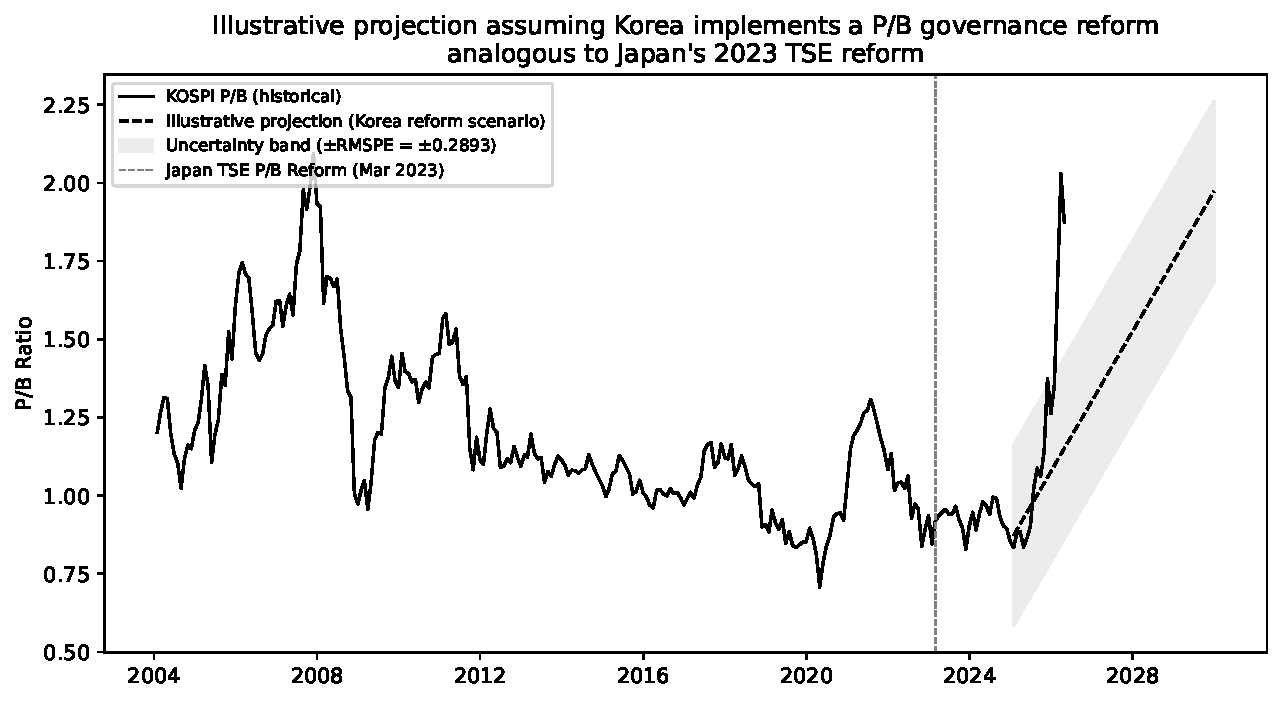
\includegraphics[width=\textwidth]{../output/figures/figure4_counterfactual_projection.pdf}
  \caption{Illustrative Counterfactual Projection: KOSPI P/B under Korea Reform Scenario.
    Solid line: KOSPI historical P/B through 2024. Dashed line: mechanical projection applying
    Japan's post-2023 synthetic-control gap slope to Korea's December 2024 P/B level. Shaded
    band: $\pm$RMSPE ($= \pm 0.1451$). This is not a forecast.}
  \label{fig:figure4}
\end{figure}

\subsection{Conclusions and Future Research}

This paper documents a persistent Korea Discount and evaluates whether Japan's governance
reform dates provide useful evidence for Korean policy design. The descriptive event-window
analysis shows large movements in the KOSPI--TOPIX P/B spread around Japan's reform dates,
including a substantial deepening of the Korea discount after the 2023 TSE P/B Reform. Because
the event-window design is saturated, overlap-prone, and reported without standard errors, it
does not provide clean causal identification. Panel OLS reform-by-Japan interaction estimates
are mixed in sign and noisy under the wild bootstrap, with $p$-values of 0.625, 0.375, and
0.500. The synthetic control assigns full weight to MSCI EM Asia (RMSPE $=0.1451$) and does
not show a sustained monotonic Japan-specific valuation premium after March 2023. The
geopolitical risk coefficient ($-0.02$, $t=-0.84$, $p=0.40$) is statistically insignificant,
consistent with geopolitical risk being priced continuously as a structural level discount
rather than through discrete monthly escalation responses.

Several directions merit future research. Firm-level panel analysis combining chaebol-specific
governance indices with market-level data would complement the country-level time-series
identification employed here. As Korea's Value-Up Program matures and generates multi-year
post-announcement data beyond the early 2024--2025 period, an event study of the Korean
program analogous to this paper's Japan analysis would provide direct causal evidence on
Korean governance reform. Extension to other discount markets --- China A-shares, India,
Gulf Cooperation Council --- would test whether the structural channels identified for Korea
generalize to other civil-law, concentrated-ownership equity markets.

\bibliographystyle{apalike}
\bibliography{references}

\begin{appendices}

\section{Variable Definitions}
\label{app:vardefs}

Table~\ref{tab:vardefs} defines the primary variables used in the analysis.

\begin{table}[htbp]
\centering
\caption{Variable Definitions}
\label{tab:vardefs}
\begin{tabular}{lp{10cm}}
\toprule
Variable & Definition \\
\midrule
P/B & Price-to-book ratio: equity market capitalization divided by the book value of equity,
  as reported by Bloomberg (\texttt{PX\_TO\_BOOK\_RATIO}) for each index at month-end. \\
P/E & Price-to-earnings ratio: equity market capitalization divided by trailing 12-month net
  earnings, as reported by Bloomberg (\texttt{PE\_RATIO}) for each index at month-end. \\
GPR & Geopolitical Risk index from \citet{caldara2022}; monthly frequency; constructed by
  aggregating newspaper coverage of geopolitical threats and escalation events. The GPRNK
  sub-index from \citet{imf2021} is used for North Korea-specific escalation. \\
Stewardship Code dummy & $D_{2014,t} = \mathbf{1}[t \geq \text{February 2014}]$; indicator
  equal to 1 for months on or after Japan's Stewardship Code adoption date. \\
CGC dummy & $D_{2015,t} = \mathbf{1}[t \geq \text{June 2015}]$; indicator equal to 1 for
  months on or after Japan's Corporate Governance Code adoption date. \\
TSE P/B Reform dummy & $D_{2023,t} = \mathbf{1}[t \geq \text{March 2023}]$; indicator equal
  to 1 for months on or after the Tokyo Stock Exchange P/B reform announcement date. \\
\bottomrule
\end{tabular}
\end{table}

All reform date indicators are derived from the dates locked in \texttt{config.py} before
any data transformation, providing a look-ahead bias firewall.

\section{Additional Robustness Tables}
\label{app:robustness}

This appendix presents four additional robustness tables. Tables~B.1--B.2 replicate the
panel OLS and descriptive event-window exercises using price-to-earnings (P/E) as the outcome
variable instead of price-to-book. The P/E results are noisier and should be interpreted as
descriptive robustness evidence rather than as a separate causal design. Tables~B.3--B.4 substitute
alternative control groups --- MSCI~EM~Asia and MSCI~EM~ex-China --- for the primary MSCI~EM
control to test whether the Korea Discount estimate is sensitive to the choice of emerging
market benchmark. The Korea Discount estimate is robust to both alternative specifications.

% Robustness table fragments
\begin{table}
\caption{Panel OLS Robustness - EM ASIA Control Group}
\label{tab:robust_alt_em_asia}
\begin{tabular}{llll}
\toprule
 & Baseline two-way FE & + reform dummies & + reform x Japan \\
term &  &  &  \\
\midrule
Post Stewardship Code &  & absorbed by time FE & absorbed by time FE \\
Post Corporate Governance Code &  & absorbed by time FE & absorbed by time FE \\
Post TSE P/B Reform &  & absorbed by time FE & absorbed by time FE \\
Stewardship x Japan &  &  & -0.01 (0.03) \\
Corporate Governance Code x Japan &  &  & -0.28 (0.04) \\
TSE P/B Reform x Japan &  &  & -0.24 (0.12) \\
\multicolumn{4}{l}{\footnotesize Note: Coefficients from two-way FE PanelOLS using robust standard errors in parentheses. Post reform dummies are absorbed by time fixed effects where noted.} \\
\bottomrule
\end{tabular}
\end{table}

\input{../output/robustness/robustness_alt_control_em_exchina.tex}
\begin{table}
\caption{P/E robustness: two-way fixed effects PanelOLS estimates of Japan reform valuation responses.}
\label{tab:robustness_pe_panel_ols}
\begin{tabular}{llll}
\toprule
 & Baseline two-way FE & + reform dummies & + reform x Japan \\
term &  &  &  \\
\midrule
post\_stewardship &  & absorbed by time FE & absorbed by time FE \\
post\_cgc &  & absorbed by time FE & absorbed by time FE \\
post\_tse\_pb\_reform &  & absorbed by time FE & absorbed by time FE \\
stewardship\_x\_japan &  &  & -32.08 [0.125] \\
cgc\_x\_japan &  &  & -0.09 [0.875] \\
tse\_pb\_reform\_x\_japan &  &  & -0.47 [0.250] \\
\multicolumn{4}{l}{\footnotesize Note: Coefficients use P/E (price-to-earnings) as the dependent variable in two-way FE PanelOLS. For \textit{+ reform x Japan} specification, bracketed values are wild-bootstrap p-values (999 Rademacher draws, clustered by country). Standard errors shown for all other estimable cells.} \\
\bottomrule
\end{tabular}
\end{table}

% P/E robustness descriptive CARs: coefficients and cumulative abnormal KOSPI-TOPIX P/E spread.
% Standard errors are not reported: the saturated cohort x relative-time design
% makes sandwich robust inference undefined. See paper text for robustness discussion.
\begin{table}
\caption{P/E stacked event-study descriptive CAR estimates (no inference reported).}
\label{tab:robustness_pe_event_study_coefs}
\begin{tabular}{lrrr}
\toprule
Event & Month & Coefficient & CAR \\
\midrule
Japan Stewardship Code (Feb 2014) & -12 & -5.80 & -5.80 \\
Japan Stewardship Code (Feb 2014) & -11 & -3.27 & -9.07 \\
Japan Stewardship Code (Feb 2014) & -10 & -1.71 & -10.78 \\
Japan Stewardship Code (Feb 2014) & -9 & -4.39 & -15.17 \\
Japan Stewardship Code (Feb 2014) & -8 & 0.25 & -14.92 \\
Japan Stewardship Code (Feb 2014) & -7 & -0.60 & -15.52 \\
Japan Stewardship Code (Feb 2014) & -6 & -0.28 & -15.80 \\
Japan Stewardship Code (Feb 2014) & -5 & 3.15 & -12.66 \\
Japan Stewardship Code (Feb 2014) & -4 & 2.43 & -10.22 \\
Japan Stewardship Code (Feb 2014) & -3 & 2.78 & -7.44 \\
Japan Stewardship Code (Feb 2014) & -2 & 3.28 & -4.16 \\
Japan Stewardship Code (Feb 2014) & -1 & 0.00 & -4.16 \\
Japan Stewardship Code (Feb 2014) & 0 & 3.20 & -0.96 \\
Japan Stewardship Code (Feb 2014) & 1 & 2.39 & 1.43 \\
Japan Stewardship Code (Feb 2014) & 2 & 5.72 & 7.15 \\
Japan Stewardship Code (Feb 2014) & 3 & 5.70 & 12.85 \\
Japan Stewardship Code (Feb 2014) & 4 & 10.02 & 22.88 \\
Japan Stewardship Code (Feb 2014) & 5 & 9.37 & 32.25 \\
Japan Stewardship Code (Feb 2014) & 6 & 9.87 & 42.12 \\
Japan Stewardship Code (Feb 2014) & 7 & 8.92 & 51.03 \\
Japan Stewardship Code (Feb 2014) & 8 & 7.82 & 58.85 \\
Japan Stewardship Code (Feb 2014) & 9 & 7.28 & 66.14 \\
Japan Stewardship Code (Feb 2014) & 10 & 13.07 & 79.20 \\
Japan Stewardship Code (Feb 2014) & 11 & 12.64 & 91.84 \\
Japan Stewardship Code (Feb 2014) & 12 & 13.20 & 105.04 \\
Japan Stewardship Code (Feb 2014) & 13 & -0.53 & 104.51 \\
Japan Stewardship Code (Feb 2014) & 14 & 2.64 & 107.15 \\
Japan Stewardship Code (Feb 2014) & 15 & 2.91 & 110.07 \\
Japan Stewardship Code (Feb 2014) & 16 & 1.70 & 111.77 \\
Japan Stewardship Code (Feb 2014) & 17 & 2.16 & 113.94 \\
Japan Stewardship Code (Feb 2014) & 18 & 1.38 & 115.31 \\
Japan Stewardship Code (Feb 2014) & 19 & 3.37 & 118.68 \\
Japan Stewardship Code (Feb 2014) & 20 & 4.79 & 123.48 \\
Japan Stewardship Code (Feb 2014) & 21 & 3.82 & 127.30 \\
Japan Stewardship Code (Feb 2014) & 22 & 3.82 & 131.12 \\
Japan Stewardship Code (Feb 2014) & 23 & 3.89 & 135.01 \\
Japan Stewardship Code (Feb 2014) & 24 & 4.64 & 139.65 \\
TSE Corporate Governance Code (Jun 2015) & -12 & 4.77 & 4.77 \\
TSE Corporate Governance Code (Jun 2015) & -11 & 3.82 & 8.60 \\
TSE Corporate Governance Code (Jun 2015) & -10 & 4.02 & 12.61 \\
TSE Corporate Governance Code (Jun 2015) & -9 & 2.76 & 15.38 \\
TSE Corporate Governance Code (Jun 2015) & -8 & 1.37 & 16.74 \\
TSE Corporate Governance Code (Jun 2015) & -7 & 0.53 & 17.27 \\
TSE Corporate Governance Code (Jun 2015) & -6 & 6.01 & 23.28 \\
TSE Corporate Governance Code (Jun 2015) & -5 & 5.28 & 28.56 \\
TSE Corporate Governance Code (Jun 2015) & -4 & 5.54 & 34.09 \\
TSE Corporate Governance Code (Jun 2015) & -3 & -8.49 & 25.60 \\
TSE Corporate Governance Code (Jun 2015) & -2 & -5.62 & 19.98 \\
TSE Corporate Governance Code (Jun 2015) & -1 & 0.00 & 19.98 \\
TSE Corporate Governance Code (Jun 2015) & 0 & -7.16 & 12.82 \\
TSE Corporate Governance Code (Jun 2015) & 1 & -7.00 & 5.82 \\
TSE Corporate Governance Code (Jun 2015) & 2 & -8.09 & -2.27 \\
TSE Corporate Governance Code (Jun 2015) & 3 & -6.40 & -8.67 \\
TSE Corporate Governance Code (Jun 2015) & 4 & -5.28 & -13.95 \\
TSE Corporate Governance Code (Jun 2015) & 5 & -6.55 & -20.50 \\
TSE Corporate Governance Code (Jun 2015) & 6 & -6.85 & -27.35 \\
TSE Corporate Governance Code (Jun 2015) & 7 & -7.09 & -34.44 \\
TSE Corporate Governance Code (Jun 2015) & 8 & -6.64 & -41.07 \\
TSE Corporate Governance Code (Jun 2015) & 9 & -9.34 & -50.41 \\
TSE Corporate Governance Code (Jun 2015) & 10 & -7.04 & -57.45 \\
TSE Corporate Governance Code (Jun 2015) & 11 & -7.25 & -64.70 \\
TSE Corporate Governance Code (Jun 2015) & 12 & -9.12 & -73.82 \\
TSE Corporate Governance Code (Jun 2015) & 13 & -7.84 & -81.67 \\
TSE Corporate Governance Code (Jun 2015) & 14 & -8.62 & -90.28 \\
TSE Corporate Governance Code (Jun 2015) & 15 & -10.03 & -100.32 \\
TSE Corporate Governance Code (Jun 2015) & 16 & -10.19 & -110.50 \\
TSE Corporate Governance Code (Jun 2015) & 17 & -11.59 & -122.09 \\
TSE Corporate Governance Code (Jun 2015) & 18 & -13.86 & -135.95 \\
TSE Corporate Governance Code (Jun 2015) & 19 & -14.41 & -150.37 \\
TSE Corporate Governance Code (Jun 2015) & 20 & -14.45 & -164.82 \\
TSE Corporate Governance Code (Jun 2015) & 21 & -17.79 & -182.60 \\
TSE Corporate Governance Code (Jun 2015) & 22 & -15.51 & -198.12 \\
TSE Corporate Governance Code (Jun 2015) & 23 & -15.00 & -213.11 \\
TSE Corporate Governance Code (Jun 2015) & 24 & -13.43 & -226.54 \\
TSE P/B Reform Request (Mar 2023) & -12 & -1.42 & -1.42 \\
TSE P/B Reform Request (Mar 2023) & -11 & 0.38 & -1.05 \\
TSE P/B Reform Request (Mar 2023) & -10 & 0.65 & -0.39 \\
TSE P/B Reform Request (Mar 2023) & -9 & 0.80 & 0.41 \\
TSE P/B Reform Request (Mar 2023) & -8 & -0.20 & 0.21 \\
TSE P/B Reform Request (Mar 2023) & -7 & 0.04 & 0.25 \\
TSE P/B Reform Request (Mar 2023) & -6 & -1.07 & -0.82 \\
TSE P/B Reform Request (Mar 2023) & -5 & -1.26 & -2.08 \\
TSE P/B Reform Request (Mar 2023) & -4 & -1.18 & -3.25 \\
TSE P/B Reform Request (Mar 2023) & -3 & 0.48 & -2.77 \\
TSE P/B Reform Request (Mar 2023) & -2 & 0.25 & -2.52 \\
TSE P/B Reform Request (Mar 2023) & -1 & 0.00 & -2.52 \\
TSE P/B Reform Request (Mar 2023) & 0 & -0.26 & -2.78 \\
TSE P/B Reform Request (Mar 2023) & 1 & 1.11 & -1.67 \\
TSE P/B Reform Request (Mar 2023) & 2 & 1.02 & -0.65 \\
TSE P/B Reform Request (Mar 2023) & 3 & 4.30 & 3.65 \\
TSE P/B Reform Request (Mar 2023) & 4 & 3.37 & 7.02 \\
TSE P/B Reform Request (Mar 2023) & 5 & 3.63 & 10.65 \\
TSE P/B Reform Request (Mar 2023) & 6 & 7.61 & 18.26 \\
TSE P/B Reform Request (Mar 2023) & 7 & 7.20 & 25.46 \\
TSE P/B Reform Request (Mar 2023) & 8 & 6.68 & 32.13 \\
TSE P/B Reform Request (Mar 2023) & 9 & 8.13 & 40.26 \\
TSE P/B Reform Request (Mar 2023) & 10 & 9.23 & 49.49 \\
TSE P/B Reform Request (Mar 2023) & 11 & 7.22 & 56.71 \\
TSE P/B Reform Request (Mar 2023) & 12 & 9.28 & 65.99 \\
TSE P/B Reform Request (Mar 2023) & 13 & 9.81 & 75.80 \\
TSE P/B Reform Request (Mar 2023) & 14 & 9.84 & 85.64 \\
TSE P/B Reform Request (Mar 2023) & 15 & 6.37 & 92.01 \\
TSE P/B Reform Request (Mar 2023) & 16 & 7.40 & 99.42 \\
TSE P/B Reform Request (Mar 2023) & 17 & 7.50 & 106.91 \\
TSE P/B Reform Request (Mar 2023) & 18 & 6.13 & 113.04 \\
TSE P/B Reform Request (Mar 2023) & 19 & 6.30 & 119.34 \\
TSE P/B Reform Request (Mar 2023) & 20 & 6.00 & 125.34 \\
TSE P/B Reform Request (Mar 2023) & 21 & 5.64 & 130.98 \\
TSE P/B Reform Request (Mar 2023) & 22 & 5.01 & 136.00 \\
TSE P/B Reform Request (Mar 2023) & 23 & 5.71 & 141.71 \\
TSE P/B Reform Request (Mar 2023) & 24 & 6.76 & 148.47 \\
\bottomrule
\end{tabular}
\end{table}


\end{appendices}

\end{document}
